\section{Auswertung}
\label{sec:Auswertung}

\subsection{Überprüfung der Bragg Bedingung}
Die Messreihe ist in Abbildung (3) dargestellt.
Betrachtet man das Maximum der Messung, ergibt sich ein doppelter Winkel von $2 \cdot \theta = (27,5 \pm 0,1)$°, also ein Bragg-Winkel von $\theta = (13,75 \pm 0,05)$°. Da für den Kristall ein fester Winkel von $14$° eingestellt wurde, sollte der Winkel bei $\theta = 14$° liegen.


\subsection{Analyse des Emissionsspektrums einer Kupfer-Röntgenröhre}
Die aufgetragene Intensität in Abhängigkeit des doppelten Winkels $2 \cdot \theta$ ist in Abbildung (4) zu sehen.
Der von links gesehen erste Peak entspricht der $K_{\beta}$-Linie, der zweite der $K_{\alpha}$-Linie.
Aus dem Grenzwinkel $\theta = 4$° wird die maximale Energie des Bremsspektrums mit Gleichung (1) und (6) bestimmt

\begin{align*}
E_{max} = \frac{hc}{2\cdot d \sin{\theta}} = 44,129 \si{\keV} .
\end{align*}

\noindent Um die Halbwertsbreite zu bestimmen werden die Winkel auf der Mitte der Peaks gemessen. 
Diese betragen bei der $K_{\beta}$-Linie
\begin{align*}
\theta_{\beta,1} = 19,845° \\
\theta_{\beta,2} = 20,315°
\end{align*}
und bei der $K_{\alpha}$-Linie
\begin{align*}
\theta_{\alpha,1} = 22,03° \\
\theta_{\alpha,2} = 22,50° .
\end{align*}
Also lauten die Halbwertsbreiten
\begin{align*}
b_{\alpha} &= \frac{\theta_{\alpha,2} - \theta_{\alpha,1}}{2} = 0,235° \\
b_{\beta} &= 0,235° .
\end{align*}

\noindent Das Auflösungsvermögen ergibt sich durch die Energiedifferenzen der gemessenen Winkel bei der Halbwertsbreite. Die Energien werden wie oben bestimmt.
\begin{align*}
\Delta E_{\theta_{\alpha}} = E_{\theta_{\alpha,1}} - E_{\theta_{\alpha,2}} = (8,207 - 8,044) \si{\keV} = 0,163 \si{\keV}. \\
\Delta E_{\theta_{\beta}} = E_{\theta_{\beta,1}} - E_{\theta_{\beta,2}} = (9,068 - 8,866) \si{\keV} = 0,201 \si{\keV}. 
\end{align*}


\noindent Um die Abschirmkonstanten zu bestimmen, muss zuerst die Energie $E_\alpha$ und $E_\beta$ berechnet werden. 
Die Maxima der beiden Peaks liegen bei den Winkeln $\theta_{\beta} = 20,156 $° und $\theta_{\alpha} = 22,344$°.
Daraus ergeben sich erneut mit Gleichungen (1) und (6) folgende Energien
\begin{align*}
E_\alpha &= 8,097 \si{\keV} \\
E_\beta &= 8,934 \si{\keV}.
\end{align*}
Mit Gleichungen (2) und (3) werden die Abschirmkonstanten für die $K_{\alpha}$-Linie und die $K_{\beta}$-Linie berechnet.
\begin{align*}
\sigma_1 &= z_{Cu} - \sqrt{\frac{E_\beta}{R_\infty}} = 3,371\\
\sigma_2 &= z_{Cu} - 2 \cdot \sqrt{\frac{R_\infty \cdot (z_Cu - \sigma_1)^2 - E_\alpha}{R_\infty}} = 13,318 \\
\sigma_3 &= z_{Cu} - 3 \cdot \sqrt{\frac{R_\infty \cdot (z_Cu - \sigma_1)^2 - E_\beta}{R_\infty}} = 28,999
\end{align*}
Dabei entspricht $\sigma_2$ der Abschirmkonstanten auf der $K_{\alpha}$-Linie und $\sigma_3$ der auf der $K_{\beta}$-Linie.

\subsection{Absorptionsspektren verschiedener Stoffe}
Die Graphen der Absorptionsspektren der Absorber 
mit Ordnungszahl $30 \leq Z \leq 50$ befinden sich in den Abbildungen xyz.
In der nachfolgenden Tabelle \ref{tab:energie2} befinden sich zu jedem Element die aus den Graphen abgelesenen Winkel
und die damit mit Hilfe Gleichung (1) bestimmten Energien.
Analog zum letzten Kapitel, werden mit den berechneten Absorptionsenergien nach Gleichung (2) die Abschirmkonstanten berechnet.

\begin{table}[H]
  \centering
  \caption{Die zu jedem Element berechneten Absorptionsenergien und Abschirmkonstanten.}
  \label{tab:energie2}
\begin{tabular}{c c c c c}
  \toprule
Element & $Z$ & $\theta \:/\: °$ & $E_\text{K}\:/\: \si{\kilo\electronvolt}$ & $\sigma$\\
\midrule
Zink & 30 & 18,6 & 9,651 & 3,36\\
Brom & 35 & 13,3 & 13,381  & 3,63\\
Strontium & 38 & 11,3 & 15,710 & 4,01\\
Zirkonium & 40 & 10 & 17,727 & 3,90\\
\bottomrule
\end{tabular}
\end{table}

\noindent Nach Gleichung (2) ist die Quadratwurzel aus der berechneten Energie $E_\text{K}$ proportional zur Ordnungszahl $Z$. So lässt sich die
Rydbergenergie durch eine Ausgleichsreichnung berechnen. Diese lineare Regression wird mittels SciPy durchgeführt und hat die Form
\begin{equation}
\label{eqn:ausgleich1}
  \sqrt{E_\text{K}}(Z) = a \cdot Z + b.
\end{equation}
Dabei entspricht der Parameter $a^2$ der Rydbergenergie und die Ausgleichsreichnung ist in Abbildung \ref{fig:ausgleich} zu sehen.
\begin{figure}[H]
  \center
  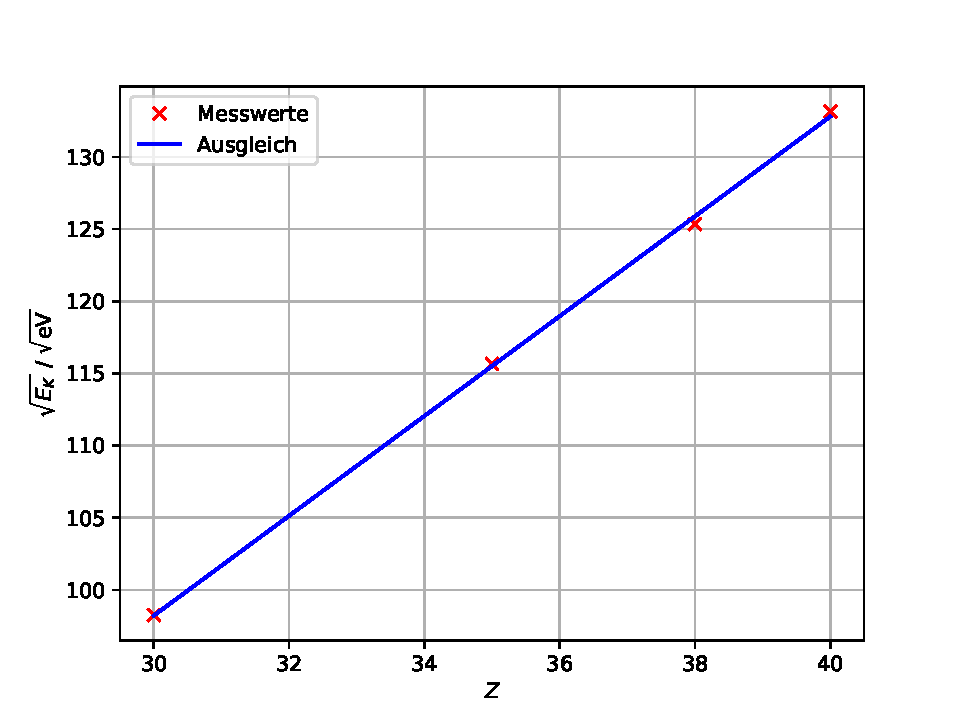
\includegraphics[scale = 0.75]{rydberg.pdf}
  \caption{Lineare Regression zur Berechnung der Rydbergenergie.}
  \label{fig:ausgleich}
\end{figure}
\noindent Die nach Gleichung \eqref{eqn:ausgleich1} berechneten Parameter sind:
\begin{align*}
a &= (\num{3.46 +- 0.06})\,\frac{1}{\sqrt{\si{\electronvolt}}} \\
b &= (\num{-5.5 +- 2.2})\,\sqrt{\si{\electronvolt}}.
\end{align*}
Mit dem direkten Vergleich zur Gleichung (2) wird der Zusammenhang deutlich:
\begin{align*}
R_\infty = a^2 = (\num{12.0 +- 0.4})\,\si{\electronvolt}.
\end{align*}

Zuletzt wird ein weiteres Mal die Abschirmkonstante $\sigma$ für ein Element mit einer Ordnungszahl $Z \geq 70$ bestimmt. In diesem Fall wurde ein Absorber des Materials
Quecksilber mit der Ordnungszahl $Z = 80$ verwendet. Das dazugehörige Absorptionsspektrum befindet sich in Abbildung xyz. Die von der $L_2$- und $L_3$-Linie abgelesenen $\theta$-Winkel
und die nach Gleichung \eqref{eqn:lambdamin} berechneten Energien befinden sich in Tabelle \ref{tab:hg}.

\begin{table}[H]
  \centering
  \caption{Die Energien der $L_2$- und $L_3$-Linie.}
  \label{tab:hg}
\begin{tabular}{c c}
  \toprule
$\theta\:/\:°$ & $E_\text{L}\:/\: \si{\kilo\electronvolt}$ \\
\midrule
12,5 & 14,222 \\
14,7 & 12,130 \\
\midrule
\multicolumn{2}{c}{Energiedifferenz $\Delta E_\text{L}: 2,092\,\si{\kilo\electronvolt}$} \\
\bottomrule
\end{tabular}
\end{table}
\noindent Die mit der Energiedifferenz $\Delta E_\text{L}$ aus Tabelle \ref{tab:hg} und mit der Gleichung (5) berechnete Abschirmkonstante $\sigma_\text{L}$ ist:
\begin{align*}
\sigma_\text{L} = 2,18.
\end{align*}
